\section{Transition networks} \label{sec:TransitionNt}

A third main group of transformations of time series into complex networks is commonly referred to as transition networks. Unlike recurrence (and other proximity-based) networks or the numerous algorithmic variants of visibility graphs, these networks are directed by definition and, hence, trace the succession of dynamical states as time proceeds. Specifically, the nodes of a transition network correspond to certain discrete states or patterns, and directed links are established if one of these nodes is followed by the other with non-zero (empirical) probability along the observed trajectory of the system under study. Mathematically, this corresponds to a Markov chain with given transition probabilities between discrete states, which can be conveniently used for constructing a weighted and directed graph \cite{Schnakenberg1976}. In this regard, the history of transition networks is closely tied to the development of the mathematical theory of Markov chains, while explicitly exploiting the topological properties of these complex networks constructed from the transition probabilities between states or patterns in dynamical systems has probably only started in the last about 15 years, initiated by the seminal work by Nicolis \emph{et~al.}~\cite{Nicolis2005}. 

While it is most common to formulate transition networks as directed and weighted graphs, it should be noted that an adjoint unweighted network representation can be easily obtained by omitting the explicit information on transition probabilities and considering those pairs of nodes (i.e., states or patterns) as being linked via an unweighted edge which exhibit non-zero mutual transition probabilities. Alternatively to considering all non-zero probabilities, one may also choose some threshold for the transition probabilities to exclude rare transitions (e.g., due to noise in deterministic dynamical systems).

In general, there are various ways to define the nodes of a transition network upon a given data set. The simplest situation is when the data themselves take only discrete values. In this case, each possible value or, more generally, each possible $m$-tuple of such values can be directly used to define a node. This results in two parameters that should be selected taking the number $K$ of discrete states, the total length $N$ of the underlying time series, and the available computational resources into account. Notably, these algorithmic parameters -- the number $m$ of states contained in each tuple and their mutual time distance $\tau$ -- are conceptually equivalent to the parameters of time delay embedding (i.e., embedding dimension and delay) in classical nonlinear time series analysis \cite{Packard1980,kantz1997}. However, unlike in most applications of time delay embedding, in the context of transition network approaches one is not necessarily interested in having statistically independent states in the considered tuple, so that $\tau=1$ is often a convenient choice even in case of serially dependent data sequences. It should be noted that the idea of considering tuples of discrete data allows a straightforward generalization of the transition network approach to multivariate series by combining, e.g., simultaneous values of the individual univariate component time series for defining a certain node.

In the more common case of variables with continuous distributions, obtaining discretized states requires some initial transformation from continuous to discrete data, which is commonly referred to as symbolic encoding. Although this encoding results in a loss of information on the detailed state of the system under study, proper encodings minimize this loss (up to zero if using so-called generating partitions of the system under study). After having performed this discretization, one may proceed as in the case of originally discrete-valued time series.

In summary, transforming a time series into a transition network representation is a (possibly two-step) process of mapping the temporal information into a Markov chain to obtain a compressed or simplified representation of the original dynamics. In the following, the individual steps for constructing and analyzing different types of transition networks will be described in full detail.

\subsection{Symbolic encoding}\label{sec:symbolic}

Symbolic encoding transforms a time series into a set of $K$ discrete states or patterns (``symbols") $\{\pi_1, \dots , \pi_K \}$. Therefore, when analyzing time series of a variable with continuous distribution, the first step towards constructing a transition network representation is applying a suitable discretization of the considered series. 

In general, there is a well-developed theory of using symbolic sequences in the context of nonlinear time series analysis \cite{Daw2003,Finn2003,Amigo2010}, which draws upon methodological concepts like entropies and complexity measures derived upon them, commonly originating from the field of statistical mechanics and information theory. Notably, there is generally a large freedom of defining different kinds of symbolizations for an underlying time series. For deterministic discrete-time dynamical systems, there exist so-called generating partitions, in which case there is a direct correspondence between the observed trajectory and the resulting symbolic sequence that is unique up to a set of measure zero \cite{Grassberger1985,Christiansen1996,Christiansen1997}. While using such generating partitions would be desirable in many applications, their estimation from real-world data commonly poses a challenging problem \cite{Kennel2003,Hirata2004,Buhl2005}. For this purpose, in practice simplified symbolization strategies are commonly employed:

\begin{itemize}

\item Coarse-graining of phase space, sometimes also referred to as \emph{static encoding} \cite{Donner2008}, classifies the data into $K$ different groups based on intervals defined by a set of pre-defined threshold values $\{\xi_1,\dots,\xi_{K-1}\}$. In this case, symbols $\pi_q$ with $q=1,\dots,K$ are assigned according to the group membership of the respective data value (i.e., $\pi_p=q$), and
\begin{equation}
\xi_i=\left\{
\begin{array}{ll}
1 & \quad \mbox{if} \quad x_i < \xi_1, \\
q & \quad \mbox{if} \quad \xi_{q-1} \leq x_i < \xi_q \quad \mbox{for} \quad 1<q<K-1), \\
k & \quad \mbox{if} \quad x_i \geq \xi_{K-1}.
\end{array} \right.
\end{equation}

\item While the coarse-graining approach relies solely on the amplitudes of each individual data value, different types of \emph{dynamic encodings} can be defined as alternatives. One simple way consists of thresholding the difference-filtered time series of order $p$, whereby the difference filtering operator is recursively applied as
\begin{eqnarray}
\Delta^{1}x_i &=& x_{i+1}-x_i \\
\Delta^{p}x_i &=& \Delta^{p-1}x_{i+1}-\Delta^{p-1}x_i \quad (p>1).
\end{eqnarray}
\noindent
Most commonly, one uses this specific approach for obtaining some binary encoding, i.e., $\xi_t=\Theta(\Delta^{p}x_t)\in\{0,1\}$ with $\Theta(\cdot)$ being again the Heaviside function. One important variant of this approach is considering order relationships among subsequent data values in subsets of $m$ observations defined based upon the first-order difference filtered series as described above. This approach results in a symbolic encoding into $2^{m-1}$ different states representing coarse-grained local dynamical patterns. In the following, we will call this type of symbolization \emph{order-pattern based encoding}.

\item Conceptually related to the aforementioned encoding based on the \emph{pair-wise} inter-comparison between subsequent values is \emph{group-wise} ordering of values within sets of $m$ subsequent observations. Neglecting possible ties, we assign each value $x_i$ within such a sequence its local rank order $r_i\in\{1,\dots,m\}$. Notably, there will be $m!$ possible permutations of such rank order sequences, which are enumerated to obtain a symbolic encoding. This strategy allows utilizing statistical techniques like permutation entropies \cite{Bandt2002} commonly referred to as \emph{ordinal time series analysis} methods \cite{bandt2005}. Accordingly, we will refer to such permutation-based symbolizations as \emph{ordinal pattern based encoding} or simply \emph{ordinal encoding}.

\end{itemize}

While the three general strategies for symbolic encoding of time series values described above are quite common in nonlinear time series analysis, they are not exhaustive. Other types of encodings, as well as mixed strategies \cite{Donner2008}, are possible as well, depending on the specific aspects of dynamics one wishes to highlight when performing the symbolization. In this regard, there is commonly no ``optimal'' symbolization strategy for a given time series \cite{Bollt2001}, but rather great flexibility according to the dynamical features or time-scales of interest as well as the available computational resources. In general, symbolic encoding performs a natural coarse-graining of the dynamics of the system under study, which preserves essential dynamical information. Such a strategy naturally addresses common issues in many real-world time series, such as the presence of noise or intrinsic multi-stability. 

Based upon the accordingly discretized time series, a variety of relevant dynamical properties can be conveniently estimated, including symbolic correlation functions \cite{Lee1997}, mutual information \cite{Li1992}, permutation entropy \cite{Bandt2002}, or transfer entropy \cite{Staniek2008}. In most cases, the choice of the symbolization strategy and its possible algorithmic parameters (e.g., number and location of thresholds, length of considered subsets, etc.) affects the resulting estimates. For example, mutual information estimators obtained from groups with equal probabilities are commonly more reliable than such from groups of equal interval size. Since defining symbols with equal probability of occurrence can be challenging in case of other than threshold-based encodings, this observation poses natural restrictions to the interpretation of quantitative values of many statistical characteristics of symbolic sequences. 

Instead of considering statistics based upon the (joint) probability distributions of individual symbols, it is often useful to combine sequences of symbols into ``words'' of a given length $m$, which allow not only for looking at the coarse-grained state of the system under study, but rather a succession of several of such states, thereby conserving some information on its dynamics. Among the quantities that can be estimated from statistics upon such sequences, the source entropy of the underlying system is often approximated by the limit of the \textit{conditional block entropies} $s_m=S_{m+1}-S_m$ for $m\to\infty$ where
\begin{equation}
S_m=-\sum_{p=1}^{K^m} p_p^{(m)}\log p_p^{(m)}
\end{equation}
\noindent
are the block entropies, i.e., the Shannon entropies of symbolic sequences of length $m$, with $p_q^{(m)}$ being the probabilities of occurrence of all possible subsequences (words) of this length (enumerated by the index $p$) within the time series \cite{Daw2003,Ebeling1992}. Moreover, the statistical properties of the sequence distributions can be used for defining various measures of complexity \cite{Grassberger1986,Rosso2007}. Last but not least, investigating the properties of forbidden symbols and words (i.e., values or patterns that are not observed during the system's dynamical evolution) have recently attracted particular attention \cite{Amigo2007,Carpi2010}.


\subsection{Markov chains}

After having defined suitable symbols or words, which are taken from an alphabet $\mathcal{A}$ of $\omega$ discrete values, the next step towards constructing a transition network representation upon a given time series is to explicitly use the temporal order of the accordingly coarse-grained observations to represent the dynamics of the observed system. 
For this purpose, we consider the transition probabilities $w_{pq} = p (\xi_{i+1} = \pi_q | \xi_i = \pi_p)$ between subsequent symbols (words) to define a weighted and directed transition network with the weight matrix $\mathbf{W} = \{w_{pq} \}, p,q \in [1, \dots, \omega]$. Note that because of $\sum_{q=1}^{\omega} w_{pq}=1$ for all $p\in\mathcal{A}$ by definition (conservation of probability), $\mathbf{W}$ is a column-stochastic matrix.

In the terminology of stochastic processes \cite{Nicolis2005}, the resulting transition networks describe a Markov chain with the nodes representing some set of states that encode the time series' amplitudes or local variations, and directed and weighted edges indicating the temporal succession of such states or patterns. Specifically, Markov chains are memoryless stochastic processes, implying that the state of the process at some time $i$ depends solely on its previous state at $i-1$. If approximating the coarse-grained dynamics of a time series as such a Markov process, this implies that the $n$-step transition probabilities are simply given by the entries of $\mathbf{W}^n$. It should be emphasized, however, that trajectories of dynamical systems commonly exhibit serial correlations, so that this simplifying approximation is commonly not suitable for fully describing the longer-term dynamical evolution of the system. Nonetheless, the Markov chain analogy allows reconsidering terms like absorbing or recurrent states or stationary densities in terms of transition network properties. Specifically, absorbing states of a Markov chain can be identified as transition network nodes with zero out-degree (respectively, zero out-strength), since $w_{pq}=\delta_{pq}$. Recurrent states are characterized by their membership in loops of length greater than one, while the stationary density is given as the eigenvector of $\mathbf{W}$ with eigenvalue 1, which is unique in case of non-degenerated Markov chains. This implies a close connection with the network measure of eigenvector centrality.

It should be emphasized that the duality between Markov chains and transition networks holds for any Markov chain irrespective of the existence of an underlying time series.


	\subsection{Coarse-graining based transition networks}\label{sec:cgtn}

	The construction of coarse-graining based transition networks draws upon a proper phase space partition. For instance, we first mesh the $d$-dimensional phase space with boxes of equal size following the traditional idea of fractal dimension computations \cite{Grassberger1983PRL,Grassberger1983PLA} or complexity measures \cite{Crutchfield1989}. When working with univariate time series, $d=m$ (i.e., the length of the considered symbolic sequences). An alternative, mathematically preferable yet harder to construct alternative would be a separation into boxes with equal probability \cite{Liu2016}. Then, each box $p$ is labeled with the symbol $\pi_p$ and regarded as a vertex in the network. The connectivity between two boxes (nodes) $\pi_p$ ($p$) and $\pi_q$ ($q$) is then represented by the empirical transition frequency following the temporal order of observations. 

	The transition probability approach is well suited for identifying such ``states" (i.e., regions in phase space) that have a special importance for the dynamical evolution of the studied system, for example, in terms of their betweenness centrality $b_p$ or similar measures. Moreover, the resulting networks do not only depend on a single parameter, but on the specific definition of the full set of classes. Note, however, that coarse graining might be a valid approach in case of noisy real-world time series, where extraction of dynamically relevant information hidden by noise can be supported by grouping the data. In contrast to the other approaches for constructing complex networks from time series, the topology of transition networks depends on the specific choice of discretization. 

	For a trajectory that does not leave a finite volume in phase space, there is only a finite number of discrete ``states" $\pi_p$ with a given minimum size in phase space. This implies the existence of absorbing and/or recurrent states in the associated Markov chain. Specifically, in case of dissipative dynamics, the phase space segments corresponding to absorbing and recurrent nodes provide a coarse-grained description of the system's attractor(s).
		
		It should be noted that unlike in visibility graphs and related methods, detailed temporal information is lost at the network level after the coarse graining since the transition frequency matrix $\mathbf{W}$ is estimated over the entire time series. Therefore, the resulting transition network is a static representation of the system's dynamics, which requires the system to be stationary and ergodic. Violation of the stationarity assumption could imply the transition matrix $\mathbf{W}$ being explicitly time-dependent, which however would make a proper estimation of its coefficients challenging if only a single time series is available as a realization of the non-stationary system dynamics. In this context, Weng {\emph {et al.}} \cite{Weng2017} proposed constructing a temporal network from time series by unfolding temporal information into an additional topological dimension. More specifically, a transition from node $p$ to $q$ is established whenever the trajectory flow performs a transition from $p$ to $q$ at time $t_i$ which is denoted as ($p \to q; i$). By adding the additional time axis to the transition route, the consecutive memory network is constructed by introducing a memory factor. Weng {\textit{et al.}} further proposed memory entropy analysis to characterize the memory effect in the observed time series. The identified memory effect can accurately differentiate between various types of time series including white noise, $1/f$ noise, AR model, periodic and chaotic time series. 

In general, there is a close analogy between coarse-graining based transition networks and Lagrangian flow networks \cite{Lindner2017,Donner2019} used for describing structural characteristics of flows. The latter type of network representations has been originally introduced for studying geophysical flows in the atmosphere and ocean \cite{Rossi2015,Ser-Giacomi2015}, but can also be applied for investigating the behavior of dynamical systems in their underlying phase space. Moreover, for nonlinear maps or ordinary differential equations, an equivalent transformation has also been termed \emph{Ulam networks} \cite{Shepelyansky2010,Ermann2010,Chakhmakhchyan2013,Ermann2015,Frahm2018} in parts of the literature, referring to the estimation of transition probabilities of trajectories between finite boxes being known as Ulam's method. While the main difference with respect to the transition networks used for the purpose of time series analysis is that Lagrangian flow networks and Ulam networks encode transition probabilities between volume elements that are commonly based on the observation of the trajectories of ensembles of tracer particles that are passively advected within a given flow field, in case of stationary and ergodic systems, results obtained for flow networks can be directly translated to transition networks in the asymptotic limit. Specifically, it has been demonstrated that node properties like degree, eigenvector centrality, or cutoff closeness have a close correspondence with spatial patterns of finite-time Lyapunov exponents or entropies (highlighting the positions of invariant manifolds of hyperbolic trajectories of the system under study) \cite{Ser-Giacomi2015,Lindner2017}. Other dynamically relevant structures like elliptic fixed points and periodic orbits can be identified by different network properties like the local clustering coefficient \cite{Rodriguez-Mendez2017}.


		\subsubsection{Ordinal pattern transition networks for univariate time series} \label{sec:OPtransition}
		As an alternative to phase space partitioning, one may define the node set of a transition network based on some different symbolic representation of the studied time series, for instance, ordinal patterns \cite{Li2008,McCullough2015}. This strategy has been followed recently in a growing number of studies \cite{Small2013,McCullough2015,Kulp2016b,McCullough2017b,Small2018}. Among others, a series of systematic investigations of ordinal methods has been conducted on irregularly sampled time series \cite{Kulp2016a,McCullough2016,Sakellariou2016}, which shows great potentials for studies of experimental observation data from climate sciences. 

		To construct an ordinal pattern transition network (OPTN), the first step is to embed the given one-dimensional time series $\{x_i\}$ by using traditional time delay embedding with a proper choice of embedding dimension $m$ and time delay $\tau$. Then, embedded points in phase space are mapped to nodes in the network space according to the sequence of rank orders, and links are allocated between nodes based on temporal succession on the trajectory. In Fig.~\ref{fig:rosTNm}, we show an example of an OPTN using the algorithm of \cite{McCullough2015}. 
\begin{figure}[ht]
	\centering
	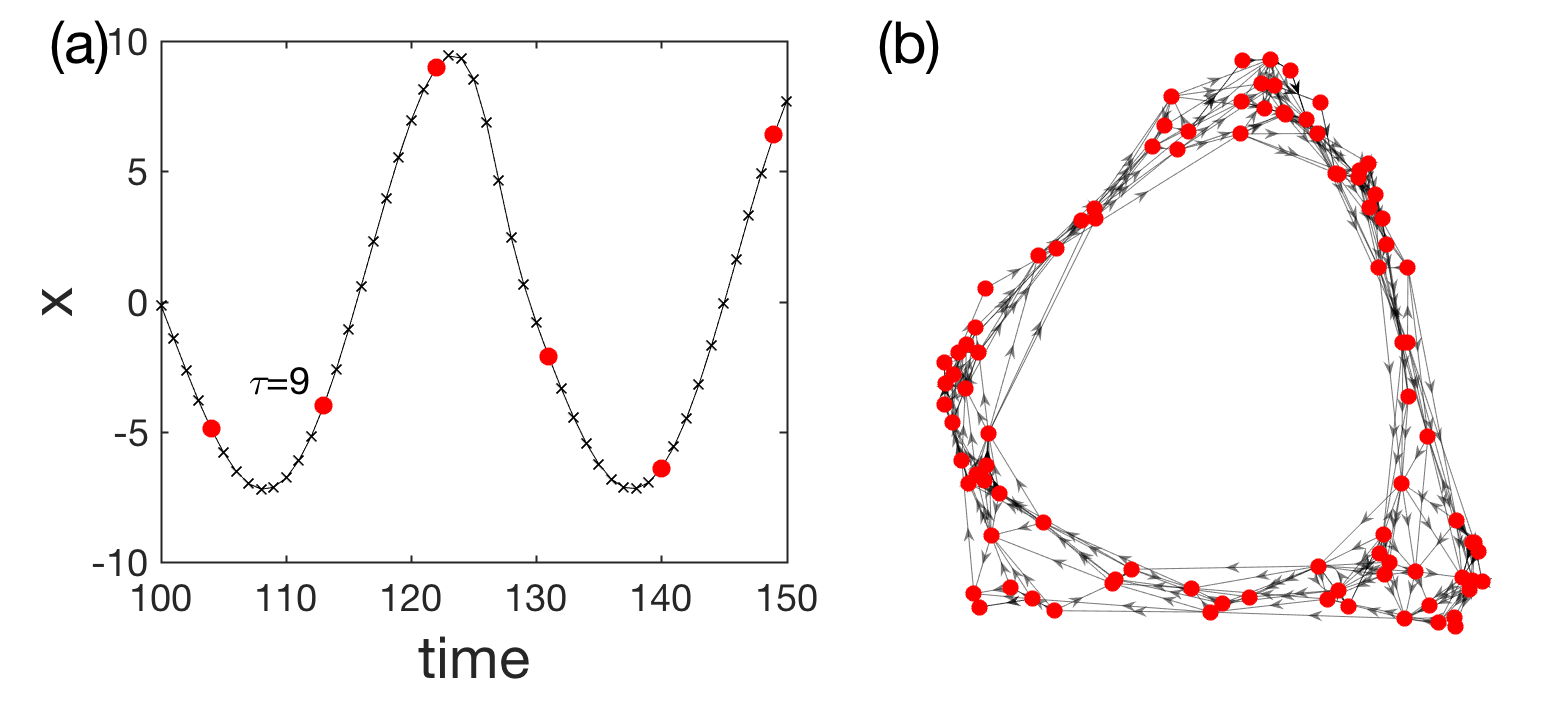
\includegraphics[width=\columnwidth]{Chapter05_TransitionNt/rosslerOPexample.eps}
\caption{(a) Illustration of permutation symbols from a time series of the R\"ossler attractor ($a = 0.165$ in Eq.~\eqref{eq:roessler}). Assume $\tau = 9$ and $m = 6$. One embedded state vector $\vec{x}_{104} = \{x_{104}, x_{113}, x_{122}, x_{131}, x_{140}, x_{149} \}$ is highlighted by red color, and its corresponding pattern is defined by the rank ordering $\pi_{104} = \{5, 1, 2, 4, 6, 3\}$. (b) Resulting OPTN (isolated vertices and self-loops are excluded in the visualization). Directed edges are indicated by arrows. Reproduced from \cite{McCullough2015}. \label{fig:rosTNm}}
\end{figure}
		
		In \cite{McCullough2015}, McCullough {\textit{et al.}} illustrated the construction algorithm in detail for the R\"ossler system and found that periodic dynamics translates to ring structures whereas chaotic time series translate to band or tube-like structures -- thereby indicating that this algorithm generates networks whose structure is sensitive to qualitatively different system dynamics. Furthermore, it has been demonstrated that simple network measures (including the mean out-degree and variance of out-degrees) can track changes in the dynamical behavior in a manner comparable to the largest Lyapunov exponent \cite{McCullough2015}. Therefore, topological characteristics of OPTNs have the potential to provide useful indicators for dynamical discrimination of different states and the detection of change points. 
		
		Measures of transitional complexity have been further proposed in \cite{McCullough2017b} to quantify the resulting OPTNs. Based on the transition matrix $\mathbf{W}$ of an OPTN that excludes the possibility of self-loops, McCullough {\textit{et al}} \cite{McCullough2017b} considered the local out-link transition frequency between the ordinal patterns $\pi_p$ and $\pi_q$
		\begin{equation} \label{eq:localTp}
			p_{pq} = \left \{ \begin{aligned}
							& 0,  \;\;\;\;\;\;\;\;\;\;\; \text{if} \; p = q\\
							& \frac{w_{pq}}{\sum_{q, q \neq p} w_{pq}} \;\;\;\;\;\; \text{if} \; p \neq q.\\
							\end{aligned}
					    \right.
		\end{equation}
		Note that the transition frequency of Eq.~\eqref{eq:localTp} is pattern (row-) wise normalized. Then, the Shannon entropy of each row of Eq.~\eqref{eq:localTp} gives the \emph{local node out-link entropy} $s_{p}^{L} = -\sum_{q} p_{pq} \log p_{pq}$. By averaging over the network, we obtain the expected value of the transitional complexity, which is called \emph{global node out-link entropy} 
		\begin{equation}\label{eq:globalTp}
			S^{GNE} = \sum_{p} p_p s_{p}^{L}. 
		\end{equation}
		The lower bound $S^{GNE} = 0$ implies that there is no uncertainty in the system, which corresponds to time series that are strictly monotonic or have a strictly periodic series of ordinal patterns. Further, an infinitely long time series of uniform independent and identically distributed noise yields the upper bounds for $S^{GNE}$ \cite{McCullough2017b}. 
		
		Embedding dimension $m$ and time delay $\tau$ are two important parameters in the construction of OPTNs, having crucial impacts on the appearance of forbidden order patterns \cite{Kulp2016b,McCullough2016,Sakellariou2016}. The selection of time delay $\tau$ must be performed in relation to the sampling rate for continuous systems. Sun \emph{et al.}~\cite{Sun2014} proposed using a time delay $\tau > 1$. In \cite{McCullough2015}, the authors recommended to select these two parameters by traditional methods used for time series embedding, for instance, the first root of the autocorrelation function of the underlying time series, because it provides a sufficiently good phase space reconstruction of a deterministic dynamical system. While there does not yet exist a robust metric for determining the correct choice of $m$, for time series of the R\"ossler system they found that networks with the most visually intuitive structure often coincide with maxima of the degree variance in dependence on $m$. In addition, it was demonstrated that the range $6 \leq m \leq 10$ was the most useful when using simple network measures to track changes in the dynamics \cite{McCullough2015}. Note that the choice of $m$ also determines the level of simplification of the original phase space by ordinal partitions. 
		
Based on similar considerations, Masoller \emph{et~al.}~\cite{Masoller2015} introduced an alternative set of entropic quantifiers. Specifically, they assigned each node of an OPTN from a univariate time series a weight $w_q$ according to the probability of occurrence of the corresponding pattern, and studied the Shannon entropy of the distribution of these node weights,
\begin{equation}
\mathcal{S}^P=-\sum_{p=1} p_p \log p_p
\end{equation}
\noindent
which corresponds to the classical permutation entropy, together with the local per-node entropy and network-averaged node entropy,
\begin{equation}
\mathcal{S}_p=-\sum_{q} w_{pq}\log w_{pq} \ \mbox{and} \ \mathcal{S}^N = \frac{1}{\omega} \sum_{p=1}^\omega \mathcal{S}_p.
\end{equation}
\noindent
In addition, they studied the \emph{asymmetry coefficient}
\begin{equation}
a=\frac{\sum_p \sum_{q\neq p} \left| w_{pq}-w_{qp} \right|}{\sum_p \sum_{q\neq p} \left( w_{pq}+w_{qp} \right)},
\end{equation}
\noindent
which takes values between $a=0$ (for a completely symmetric network) and $a=1$ (in a fully directed network where each link between any pair of nodes is completely unidirectional). Masoller \emph{et~al.}~\cite{Masoller2015} demonstrated that the aforementioned quantities trace well the succession of qualitatively different dynamical states in bifurcation scenarios of paradigmatic model systems like logistic map or tent map, as well as in real-world data from semiconductor laser experiments.

        
		\subsubsection{Order pattern transition networks for multivariate time series}
		Most recent works have focused only on univariate time series $\{x_i\}$, while the generalization to multivariate time series has remained largely untouched. However, many phenomena in the empirical sciences are of a multivariate nature. For instance, different assets in stock markets are often observed simultaneously and their joint development is analyzed to better understand tendencies. In climate science, multiple observations (temperature, pressure, precipitation, human activities, etc., from different locations) are the basis of reliable predictions of upcoming meteorological conditions. 
		
		Zhang \emph{et~al.}~\cite{Zhang2017b} proposed constructing OPTNs from multivariate (high dimensional) data. Recall that given a scalar time series $\{x_i\}$ which is produced by a deterministic dynamical system, the order structure depends on the embedding dimension $m$ and delay $\tau$. Let us start with embedding dimension $m = 2$. Neglecting equality, we have two relations between $x_i$ and $x_{i+\tau}$, namely, two symbol sequences representing order patterns $\pi_{x}$:
\begin{equation} \label{piX2D_eq}
\pi_{x,i} =  \begin{cases}
 1 & \text {if} \; x_i < x_{i+\tau}, \\
 0 & \text {if} \; x_i > x_{i+\tau}. 
\end{cases}
\end{equation}
In \cite{Small2013}, Small {\textit{et al.}} used a fixed lag $\tau = 1$ for embedding, and we adopt this idea in the following. In this case, the order pattern $\pi_x^{1}=1$ captures an increasing trend, respectively, $\pi_x^{0}=0$ corresponds to a decreasing trend of the time series. This definition is equivalent to considering the signs of the increments $\Delta x_i = x_{i+1} - x_i$ by a first-order difference of the original series. 

		Generalizing the aforementioned idea to the case of three-dimensional time series $(x_i, y_i, z_i)$, we first obtain the increment series $(\Delta x_i, \Delta y_i, \Delta z_i)$. Then the order patterns are defined by the combinations of signs of $\Delta x_i$, $\Delta y_i$ and $\Delta z_i$. In particular, the ordinal patterns $\Pi_i \in (\pi_1, \cdots, \pi_K)$ (with $K = 8$) of a three-dimensional time series are summarized in Tab.~\ref{tab:3D}. 
\begin{table}
\centering
\begin{tabular}{|c|c|c|c|c|c|c|c|c|}
\hline
$\Pi$      & $\pi_1$ & $\pi_2$ & $\pi_3$ & $\pi_4$ & $\pi_5$ & $\pi_6$ & $\pi_7$
& $\pi_8$\\
\hline
$\Delta x$ & $\pi_x^{1}, + $ & $\pi_x^{1}, + $ & $\pi_x^{1}, +$ &
$\pi_x^{1}, +$ & $\pi_x^{0}, - $ & $\pi_x^{0}, - $ &
$\pi_x^{0}, -$ & $\pi_x^{0}, -$\\
\hline
$\Delta y$ & $\pi_y^{1}, + $ & $\pi_y^{1}, + $ & $\pi_y^{0}, -$ &
$\pi_y^{0}, -$ & $\pi_y^{1}, + $ & $\pi_y^{1}, + $ &
$\pi_y^{0}, -$ & $\pi_y^{0}, -$\\
\hline
$\Delta z$ & $\pi_z^{1}, + $ & $\pi_z^{0}, - $ & $\pi_z^{1}, +$ &
$\pi_z^{0}, -$ & $\pi_z^{1}, + $ & $\pi_z^{0}, - $ &
$\pi_z^{1}, +$ & $\pi_z^{0}, -$\\
\hline
\end{tabular}
\caption{Order patterns in three-dimensional time series $(x_t, y_t, z_t)$. 
\label{tab:3D}}
\end{table}
More generally, the size of the alphabet describing the order patterns $\Pi_i$ for an $n$-dimensional time series $(\{x_{1,i}\}, \ldots, \{x_{n,i}\})$ is $m = 2^{n}$ since each component has either increasing or decreasing trend at time $i$. 

		We emphasize that multivariate OPTNs consider the increments between two consecutive time points of each one-dimensional measurement series in the space of multivariate measurements, which captures the dynamical properties of the multivariate time series in its associated ``velocity space'' (difference space). Therefore, the time delay $\tau$ in the order pattern definition (Eq.~\eqref{piX2D_eq}) has a rather different interpretation than the time delay that is often used in classical time delay embedding. The above discussion can be directly generalized to the case of $\tau>1$ and embedding dimension $m>2$ for each variable. The resulting OPTN utilizes discretized approximations of the local nullclines (i.e., $\Delta x=0$, etc.) to obtain a symbolic partitioning of the systems. In Fig. \ref{fig:rosslerTwoA}(a), the chaotic R\"ossler system is color-coded by the ordinal pattern partitions and the corresponding transition network in shown in Fig. \ref{fig:rosslerTwoA}b. 
\begin{figure}[ht]
	\centering
	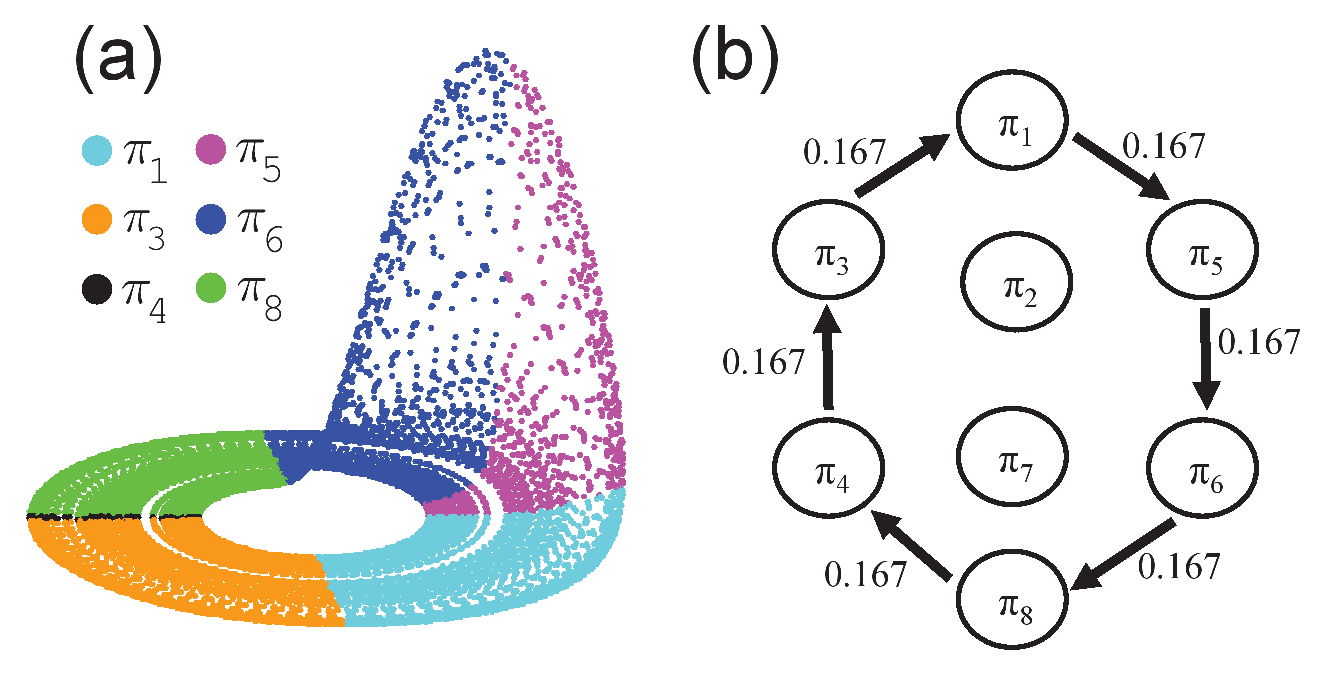
\includegraphics[width=0.7\columnwidth]{Chapter05_TransitionNt/rossler_0165N.eps}
\caption{(a) R\"ossler attractor in phase space color coded by the order patterns defined in Tab.~\ref{tab:3D} (for $a = 0.165$ in Eq.~\eqref{eq:roessler}), (b) OPTN and self-loops are excluded. Reproduced from~\cite{Zhang2017b}. \label{fig:rosslerTwoA}}
\end{figure}

In order to highlight the importance of non-self transitions between ordinal patterns, one straightforward modification of the OPTN definition would consist of removing any self-loops, which is a typical step in many applications of complex networks \cite{Costa2007}. Specifically, we can remove self-loops before computing the weight matrix $\mathbf{W}$ to keep the normalization $\sum_{p,q}^{2^n} w_{pq} = 1$. Note that in stochastic processes, self-loops can be expected not to contribute with large probabilities. 
		
		Given the empirical observations of different occurrence frequencies of ordinal patterns $p(\pi_p)$ and their mutual transition frequencies $w_{pq}$, two Shannon entropies are defined as 
		\begin{align} \label{eq:Ho}
		\mathcal{S}_O &= - \sum_{p=1}^{2^n} p(\pi_p) \log_2 p(\pi_p) , \\ \label{eq:Ht}
		\mathcal{S}_T &= - \sum_{p,q=1}^{2^{n}} w_{pq} \log_2 w_{pq}. 
		\end{align}
		In the terminologies of \cite{McCullough2017b}, $\mathcal{S}_{O}$ characterizes the vertex (node) complexity (i.e., is defined as the Shannon entropy of node weights, which is equivalent to the classical permutation entropy) and $\mathcal{S}_{T}$ the edge (link) transitional complexity, both of which have been found useful for characterizing synchronization transitions \cite{Zhang2017b}. Note that Eq.~\eqref{eq:Ht} measures the transitional complexity of the ordinal patterns, but with a slightly different normalization than that was used in \cite{McCullough2017b,Small2018}. 
		
\subsubsection{Ordinal pattern transition networks for synchronization transitions}

As a numerical application, Zhang {\textit{et al.}} \cite{Zhang2017b} constructed OPTNs to identify dynamical regimes shifts and characterize routes to phase synchronization. In particular, they considered three R\"ossler systems diffusively coupled via their $x$-components \cite{Nawrath2010} (see Eqs.~\eqref{threeRosPRL}), where $k = 1, 2, 3$ are indices for the different subsystems and $\mu$ is the coupling strength. For illustrative purposes, let us consider non-identical oscillators by choosing $\omega_1 = 0.98, \omega_2 = 1.02, \omega_3 = 1.06$ in Eqs.~\eqref{threeRosPRL}. The oscillator $k = 2$ is bidirectionally coupled to both $k=1$ and $k=3$, whereas there is no direct coupling between $k=1$ and $k = 3$. The Eqs.~\eqref{threeRosPRL} are numerically integrated by a fourth-order Runge-Kutta method with integration step $h = 0.01$. We construct OPTNs from the $x$ components, i.e., $(x_1, x_2, x_3)$, and use the definitions of patterns as summarized in Tab.~\ref{tab:3D}. The results are shown in Fig.~\ref{fig:rosslerSync}, which have been averaged over 50 random initial conditions when integrating Eqs.~\eqref{threeRosPRL}. 
\begin{figure}
	\centering
	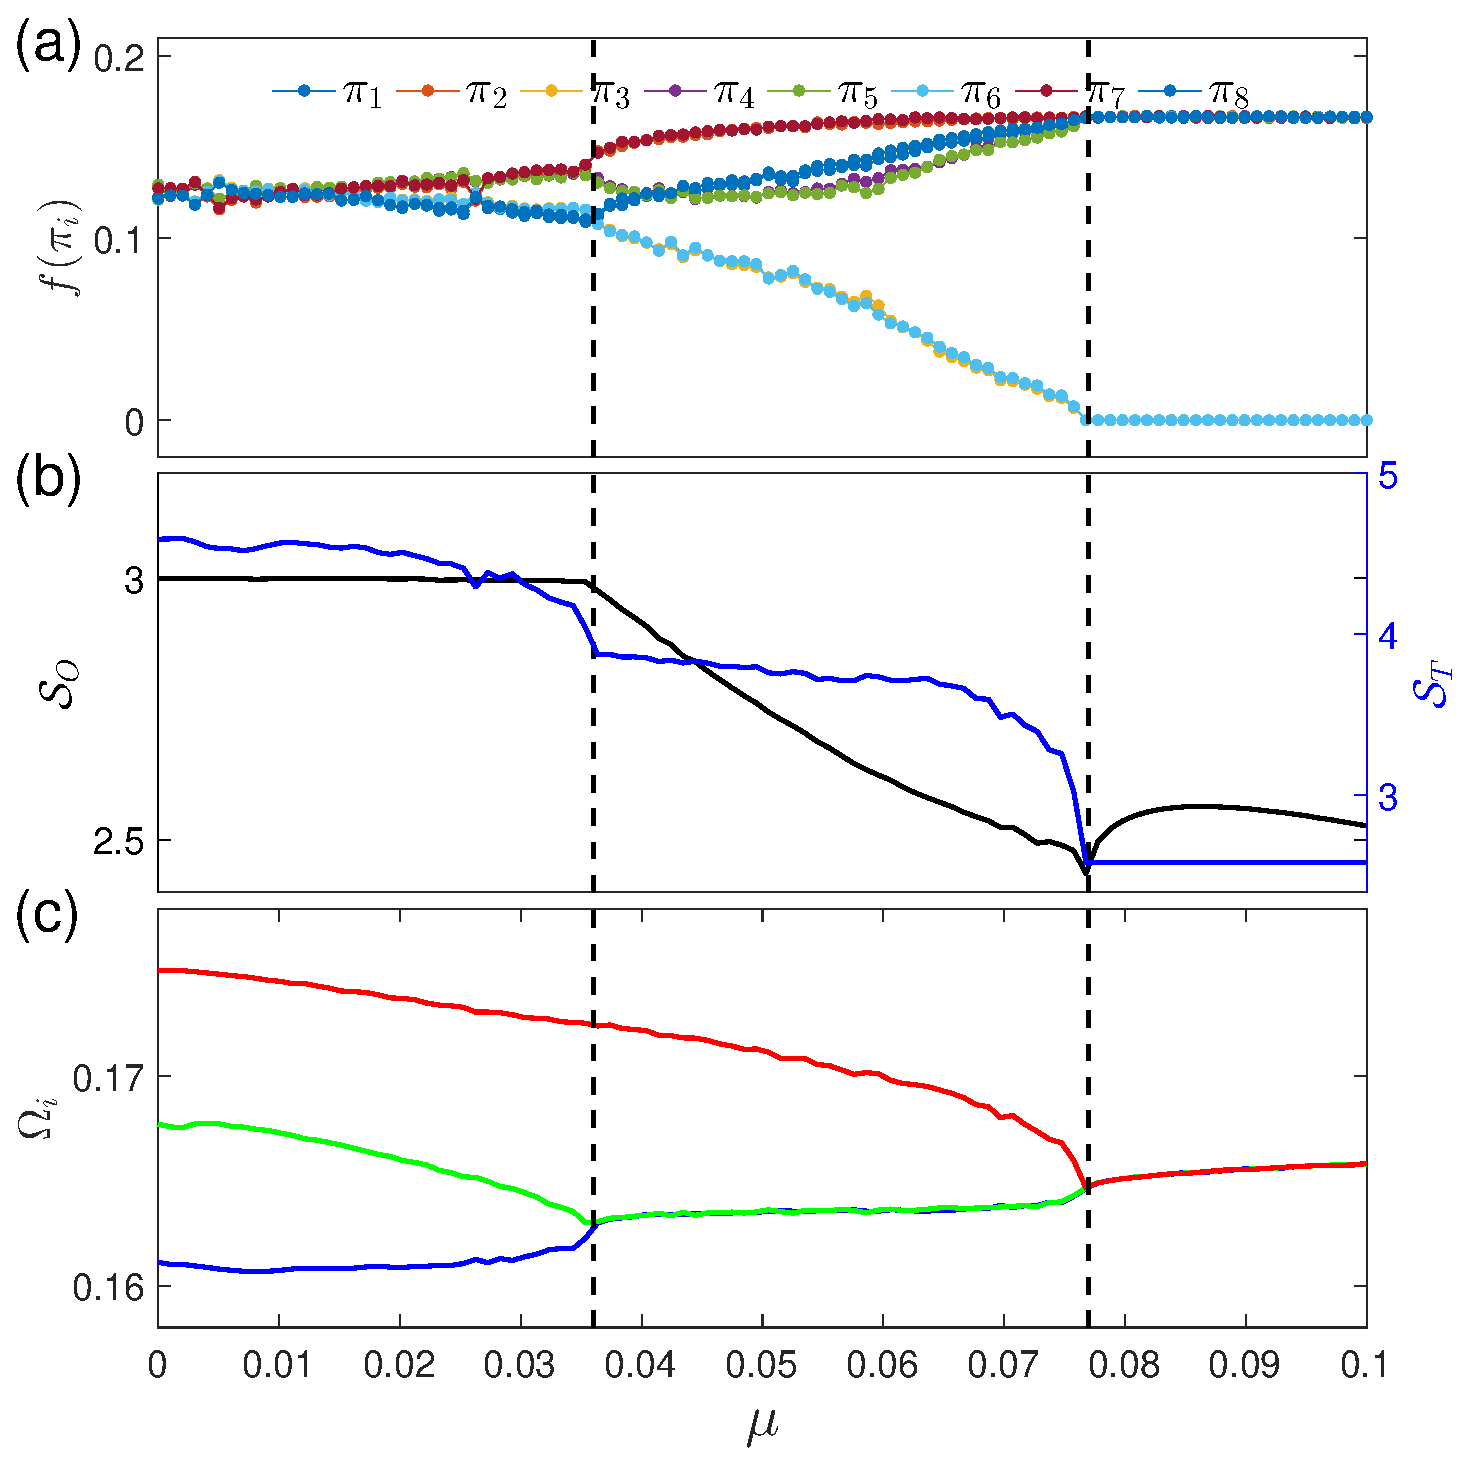
\includegraphics[width=0.6\columnwidth]{Chapter05_TransitionNt/rosslerSync.eps}
\caption{Phase synchronization transitions of three coupled R\"ossler systems. (a) Frequency of each ordinal pattern $\pi_i$, (b) entropy values $\mathcal{S}_O$ (Eq.~\eqref{eq:Ho}) and $\mathcal{S}_T$ (Eq.~\eqref{eq:Ht}), (c) mean rotation frequency $\Omega_i$ of each oscillator. Subsystem $k_1$ and $k_2$ become synchronized at $\mu_{c,1}=0.036$, and $k_3$ joins the synchronization only at a stronger coupling strength $\mu_{c.2}=0.077$. Both critical coupling values are highlighted by vertical dashed lines. Modified from~\cite{Zhang2017b}. \label{fig:rosslerSync}}
\end{figure}

\begin{figure}
	\centering
	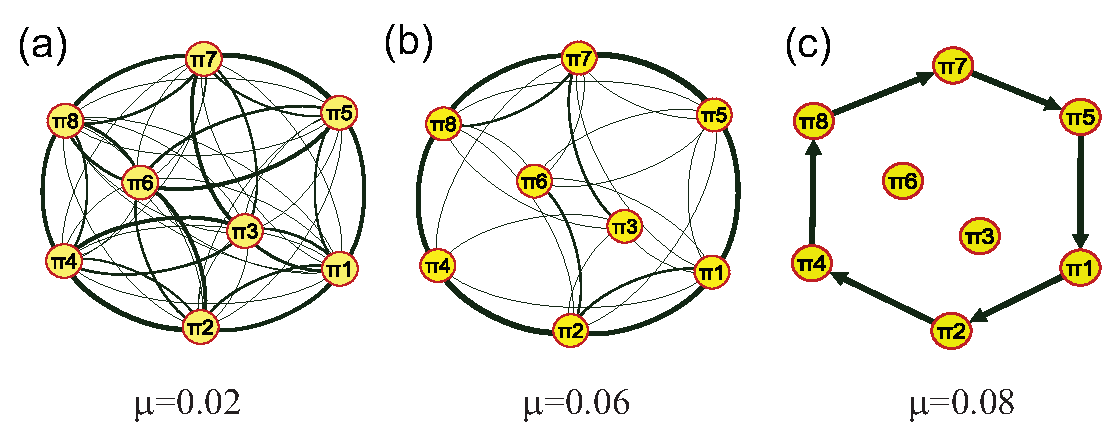
\includegraphics[width=0.8\columnwidth]{Chapter05_TransitionNt/sync_net.eps}
\caption{Ordinal transition networks on the path to phase synchronization. (a) Non-synchronized regime, $\mu = 0.02 < \mu_{c,1}$, (b) regime in which the oscillators $k=1$ and $k=2$ are phase-synchronized, but not with $k=3$, $\mu = 0.06 \in [\mu_{c,1}, \mu_{c,2}]$, (c) regime in which all three oscillators are phase locked, $\mu = 0.08 > \mu_{c,2}$. The thickness of links indicates the corresponding transition frequencies. In (a) and (b), link arrows are suppressed. Reproduced from~\cite{Zhang2017b}. \label{fig:rosslerSyncNet}}
\end{figure}

In the absence of synchrony ($\mu < \mu_{c,1}=0.036$), the three oscillators evolve almost independently such that all ordinal patterns have the same frequencies of $0.125$. There are rather small gradual changes only when $\mu$ approaches $\mu_{c,1}$ (Fig.~\ref{fig:rosslerSync}(a)). The entropy value $\mathcal{S}_T$ is sensitive to these gradual changes by showing a pronounced downward trend, while $\mathcal{S}_O$ stays about constant (Fig.~\ref{fig:rosslerSync}(b)). The average rotation frequencies $\Omega_k$ of all three oscillators are shown in (Fig.~\ref{fig:rosslerSync}(c)), which confirms the absence of synchrony in this weak coupling regime.

Increasing the coupling strength, phase synchronization first appears between oscillators $k=1$ and $k=2$, but not with $k=3$ ($\mu \in [\mu_{c1}, \mu_{c2}] =[0.036, 0.077]$). In this regime, we observe monotonic increases in the frequencies of the order patterns $\pi_1$, $\pi_2$, $\pi_7$, and $\pi_8$ (Fig.~\ref{fig:rosslerSync}(a)). In addition, we find slower increases for the frequencies of patterns of $\pi_4$ and $\pi_5$, whereas those of $\pi_3$ and $\pi_6$ systematically decrease. The changes in the frequencies of order patterns are captured by both entropy values $\mathcal{S}_O$ and $\mathcal{S}_T$, showing gradual downward trends (Fig.~\ref{fig:rosslerSync}(b)) indicating a reduction in dynamical complexity of the coupled system. The average rotation frequencies $\Omega_k$ shown in Fig.~\ref{fig:rosslerSync}(c) indicate that $k=1$ and $k=2$ are phase locked to the same rotation frequency, but $k=3$ still evolves independently.

Finally, in the regime with all oscillators being phase-synchronized ($\mu > \mu_{c2} = 0.077$), we find that the frequencies of patterns $\pi_1$, $\pi_2$, $\pi_4$, $\pi_5$, $\pi_7$ and $\pi_8$ converge to the same value of $p(\pi_q) = 1/6$, while $\pi_3$ and $\pi_6$ are absent (Fig.~\ref{fig:rosslerSync}(a)). In other words, the patterns $\pi_3$ and $\pi_6$ are forbidden if all oscillators are synchronized. The entropy $\mathcal{S}_O$ shows some parabolic trend (first increasing and then decreasing slowly), while $\mathcal{S}_T$ stays constant at a value of about $2.585$ (Fig.~\ref{fig:rosslerSync}(b)). All mean rotation frequencies converge to the same value since three oscillators are phase locked (Fig.~\ref{fig:rosslerSync}(c)).

Across the transition from asynchrony to phase synchronization, the transition networks experience rather random transitions between all possible pairs of patterns to finally approach a state of transitions between a limited number of ordinal patterns as shown in Fig.~\ref{fig:rosslerSyncNet}. Specifically, as already discussed above, $\pi_3$ and $\pi_6$ are forbidden patterns if all three oscillators are synchronized.

		\subsection{Cross and joint ordinal transition networks} 
		The method of \cite{Zhang2017b} has been further generalized to construct cross and joint ordinal partition transition networks for two coupled systems \cite{Guo2018}. For this purpose, we start with an example of a single chaotic R\"ossler system as represented by three variables $(x_{1,i}, y_{1,i}, z_{1,i})$. The OPTN is constructed based on the signs of the increments of each variable, $(\Delta x_{1,i}, \Delta y_{1,i}, \Delta z_{1,i})$, where $\Delta x_{1,i} = x_{1,i+1} - x_{1,i}$, $\Delta y_{1,i} = y_{1,i+1} - y_{1,i}$, and $\Delta z_{1,i} = z_{1,i+1} - z_{1,i}$. The definition of corresponding patterns $\Pi_i \in (\pi_1, \cdots, \pi_K)$ with $K=8$ follows again the setting in Tab.~\ref{tab:3D}. 
        
		For two coupled systems, we have additional time series from the other system as represented by $\{(x_{2,i}, y_{2,i}, z_{2,i})\}$. A cross-ordinal pattern transition network (COPTN) compares the relative rates of changes between the two systems by the signs of $(\Delta x_{1,i} - \Delta x_{2,i}), (\Delta y_{1,i} - \Delta y_{2,i})$ and $(\Delta z_{1,i} - \Delta z_{2,i})$. The resulting pattern definitions of a COPTN are summarized in Tab.~\ref{tab:3DCOPT}. An example of a COPTN constructed from two coupled R\"ossler systems in a non-synchronized regime \cite{Guo2018} is shown in Fig. \ref{fig:rosCOPT}(a). 
\begin{table}[htb]
\centering
\begin{tabular}{|c|c|c|c|c|c|c|c|c|}
\hline
$\Pi$      & $\pi_1$ & $\pi_2$ & $\pi_3$ & $\pi_4$ & $\pi_5$ & $\pi_6$ & $\pi_7$
& $\pi_8$\\
\hline
$\Delta x_1 - \Delta x_2$ & $+ $ & $+ $ & $+$ & $+$ & $ - $ & $ - $ & $-$ & $ - $\\
\hline
$\Delta y_1 - \Delta y_2$ & $ + $ & $ + $ & $ -$ & $ -$ & $ + $ & $ + $ & $ -$ & $ -$\\
\hline
$\Delta z_1 - \Delta z_2$ & $ + $ & $ - $ & $ +$ & $ -$ & $ + $ & $ - $ & $+$ & $ -$\\
\hline
\end{tabular}
\caption{Pattern definitions of a COPTN. $``+"$ means a positive value while $``-"$ stands for a negative value.  \label{tab:3DCOPT}}
\end{table}

Considering the effects of the different magnitudes of the three variables, in \cite{Guo2018} the authors defined an {\emph{alternative}} COPT by replacing $\Delta x_{1,i} - \Delta x_{2,i}$ by $\Delta x_{1,i} / x_{1,i} - \Delta x_{2,i} / x_{2,i}$, respectively, $\Delta y_{1,i} - \Delta y_{2,i}$ by $\Delta y_{1,i} / y_{1,i} - \Delta y_{2,i} / y_{2,i}$, and $\Delta z_{1,i} - \Delta z_{2,i}$ by $\Delta z_{1,i} / z_{1,i} - \Delta z_{2,i} / z_{2,i}$. An example of this alternative COPTN is shown in Fig.~\ref{fig:rosCOPT}(b). Comparing Figs.~\ref{fig:rosCOPT}(a) and \ref{fig:rosCOPT}(b), this alternative COPT reflects better the non-coherent transitions between ordinal patterns since the coupling strength is in the non-synchronized regime ($\nu = 0.02$, $\mu_{21} = 0$ and $\mu_{12} = 0.01$ in Eqs. \eqref{eq:coupled_roessler}). We note, however, that normalizing by the local value of each component may result in numerical problems close to the roots of each component time series. To better account for amplitude effects in the different variables, other normalizations (like with respect to the individual components' variances or ranges) are possible but have not yet been explored systematically.
\begin{figure}
	\centering
	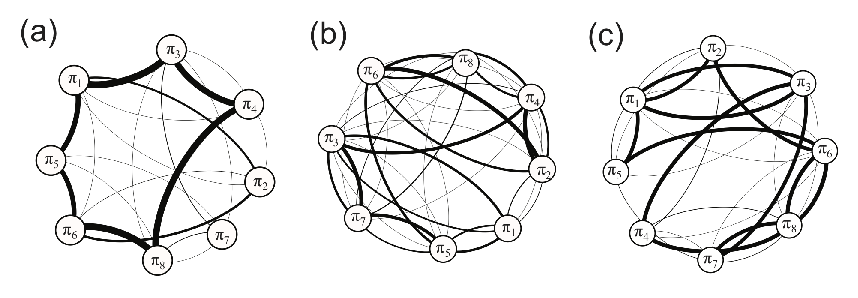
\includegraphics[width=\columnwidth]{Chapter05_TransitionNt/copt_jopt.eps}
	\caption{\small{Cross and joint OPTNs, which are reconstructed from two coupled R\"ossler systems (Eqs. \eqref{eq:coupled_roessler}) in the non-synchronized regime \cite{Guo2018}. (a) Normal cross ordinal pattern transition network (COPTN), (b) alternative version of the COPTN, and (c) joint ordinal pattern transition network (JOPTN). Link directions have been omitted in the  visualization. Reproduced from \cite{Guo2018}. } \label{fig:rosCOPT}}
\end{figure}	

Similar to the COPTN, a joint ordinal pattern transition network (JOPT) compares the relative rates of changes between two systems by the signs of $\Delta x_{1,i} \cdot \Delta x_{2,i}$, $\Delta y_{1,i} \cdot \Delta y_{2,i}$ and $\Delta z_{1,i} \cdot \Delta z_{2,i}$. The definitions of the resulting patterns are summarized in Tab.~\ref{tab:3DJOPT}. An example of a JOPTN is shown in Fig.~\ref{fig:rosCOPT}(c).
\begin{table}[htb]
\centering
\begin{tabular}{|c|c|c|c|c|c|c|c|c|}
\hline
$\Pi$      & $\pi_1$ & $\pi_2$ & $\pi_3$ & $\pi_4$ & $\pi_5$ & $\pi_6$ & $\pi_7$
& $\pi_8$\\
\hline
$\Delta x_1 \cdot \Delta x_2$ & $+ $ & $+ $ & $+$ & $+$ & $ - $ & $ - $ & $-$ & $ - $\\
\hline
$\Delta y_1 \cdot \Delta y_2$ & $ + $ & $ + $ & $ -$ & $ -$ & $ + $ & $ + $ & $ -$ & $ -$\\
\hline
$\Delta z_1 \cdot \Delta z_2$ & $ + $ & $ - $ & $ +$ & $ -$ & $ + $ & $ - $ & $+$ & $ -$\\
\hline
\end{tabular}
\caption{Pattern definitions of a JOPT. $``+"$ means a positive value while $``-"$ stands for a negative value.  \label{tab:3DJOPT}}
\end{table}
In contrast to cross ordinal patterns, we notice that the joint ordinal patterns represent whether the respective variables of two systems show the same trend of changes or not, regardless of the magnitudes of the respective variables.

The ideas of both COPTN and JOPTN have been applied to analyze synchronization transitions \cite{Guo2018}. Note that COPTN and JOPTN provide two different ways to construct networks from multivariate time series, providing complementary information. The ordinal patterns of a COPTN are defined by considering the signs of the difference $\Delta \vec{x}_1 - \Delta \vec{x}_2$ between two subsystems. In contrast, the ordinal patterns of a JOPTN are defined by the signs of the product of $\Delta \vec{x}_1 \cdot \Delta \vec{x}_2$. Notably, the amplitudes of oscillations of different variables influence directly the definition of a COPTN. However, amplitudes become practically irrelevant for a JOPTN because only the signs of the product are considered. In addition, it is straightforward to generalize the ideas of JOPTNs from two to three (or even $n$) coupled subsystems with an extended number of pattern definitions. In turn, it remains a challenge to construct COPTNs for three or more coupled subsystems. 


\subsection{Other related approaches}

		For one-dimensional symbolic sequences, one may construct a directed symbolic transition network \cite{Emmert2012}. Working with experimental data of inter-beat ($RR$) intervals of the human heart from cardiac regulations, Makowiec~\emph{et~al.} proposed to construct transitions networks from the subsequent increment series $\Delta RR_i = RR_i - RR_{i-1}$ \cite{Makowiec2013,Makowiec2013b,Makowiec2014b,Makowiec2015,Makowiec2015b,Makowiec2016}. In this series of work, they have demonstrated that transition network approaches are a powerful tool for quantifying the unique properties of the $RR$-interval time series of patients after heart transplant surgery. 
		
		When constructing OPTNs by a sliding window scheme \cite{Small2013}, the ordinal pattern of the windowed sequence corresponds to one node of the network. Since amplitude information is neglected, this approach may be combined with a transition network, where the nodes of the network are the binned amplitudes of the time series \cite{Sun2014}. More specifically, each time step $i$ is associated with a pair of symbols containing both, amplitude information $a_i$ and ordinal pattern $o_i$. The former is calculated by binning the time series in the interval $[\min_i y_i, \max_i y_i]$ into $K$ subintervals of equal size. $a_i$ is then simply the bin number associated with $y_i$. On the other hand, $o_i$ is the ordinal pattern of the embedded vector $(y_i, y_{i+\tau}, \dots, y_{i+(m-1)\tau})$. The symbol pair at step $i$, $\xi_i=(a_i,o_i)$, is then one node of the network, and it is connected by a directed link to the symbol pair $(a_{i+1},o_{i+1})$ of the successive time step. Furthermore, this algorithm has been combined with recurrence networks and surrogate networks, which has proven powerful in detecting weak nonlinearities in time series~\cite{Laut2016}. 
		
		By coarse graining of financial time series, one may focus on the particular up-down behavior associated with volatility in stock index series \cite{Li2006b,Li2007a}. More specifically, the authors of the former papers symbolize time series by using the parameter $\theta = \arctan \Delta x / \Delta t$, which characterizes the local rate of increase or decrease of the observations. Then, these local rates are coarse-grained into four states ($R, r, d, D$), which correspond to violent-up meta, common-up meta, common down meta, and violent down meta patterns, respectively. It was found that the topologically relevant nodes of the resulting transition networks play important roles in both information control and transport at the stock market \cite{Li2007a}. 
		
		In a series of works by Gao \textit{et al.}~\cite{Gao2014a,Gao2014,Gao2015}, the authors proposed a linear regression pattern transmission algorithm which captures the evolution of linear regression of bivariate time series. This algorithm has been demonstrated to be a useful tool to show the correlation mode transmission in crude oil spot price and future price \cite{Huang2015}. Based on reduced autoregressive models generated from time series, a directed transition network reconstruction algorithm has been used in \cite{Nakamura2012a}, such that the delay information has been successively captured by the transition behavior of the resulting network. In combination with proper surrogate methods, extending these ideas from a univariate to multivariate time series analysis is possible~\cite{Nakamura2016}. 
		
        Another alternative way to approach a symbolization based upon multivariate time series has been proposed by Gao \emph{et~al.}~\cite{Gao2015b}. In that paper, the authors studied the behavior of two-phase (gas--fluid) flows based on experimental observations by four conductance sensors within the two media. Starting from the corresponding acquired time series, they used a sliding window approach to estimate time-dependent correlation between all pairs of time series. A symbolic encoding has been achieved by rank-ordering the resulting six pairwise correlation coefficients. Based on the corresponding symbolization by ordinal patterns of correlation values, the authors constructed an OPTN as described above and demonstrated that corresponding network properties like weighted local clustering coefficients and closeness centralities were able to trace qualitative changes in the resulting dynamics in dependence on the gas' superficial velocity.
		
        Finally, a recent modification of transition network approaches relieves the restriction to sequences or ordinal patterns of the same degree, but rather utilizes an encoding based on optimal symbols representing sequences or patterns of variable length that form a unique alphabet for a loss-free compression of the underlying symbolic sequence \cite{Walker2018}. In the original paper, the authors employed this idea by making use of Lempel-Ziv-Welch like compression algorithm \cite{Welch1984} together with coarse-graining based transition networks constructed upon single threshold (i.e., a binary encoding). As a statistics of interest, they used the fraction of unused codewords in these \emph{coarse-graining based compression networks} and demonstrated the discriminative skills of this measure for different stochastic and chaotic model systems as well as real-world EEG data involving epileptic seizures. A more recent paper by the same authors combined the same compression algorithm with the idea of ordinal pattern based encoding and showed that considering the minimal cycle basis of the resulting \emph{ordinal compression networks} allows for testing for time irreversibility of the underlying time series.
        
